% SC3010 --- Chapter 6: Network Security
% No \documentclass --- this file is \include'd by main.tex (book class).
\chapter{Network Security: Firewalls, IDS/IPS, TLS and VPNs}
\label{ch:network}
\begin{quote}
\emph{``The network is the adversary's highway.''} --- Packets cross untrusted hops; we decide what crosses the boundary, what we notice, and how we keep it confidential while in transit.
\end{quote}

\noindent\fbox{\parbox{\dimexpr\linewidth-2\fboxsep-2\fboxrule}{%
\textbf{From zero: where we are in the story.} Ch.~5 secured the program; now we secure the wire. Every packet is an untrusted letter: the header is the envelope, the payload is the contents. This chapter asks four questions from first principles: what to drop at the gate (firewalls), what to watch for inside (IDS/IPS), how to whisper so only the intended reader hears (TLS), and how to build a private tunnel over a public road (VPNs).
}}

\section*{Learning Outcomes}
After this chapter you will be able to:
\begin{enumerate}[label=(L\arabic*)]
    \item compare packet-filter, stateful, and application-layer firewalls and write a rule set;
    \item contrast signature-based vs.\ anomaly-based detection and explain IDS vs.\ IPS placement;
    \item describe the TLS~1.3 handshake, key schedule, and why it provides forward secrecy;
    \item distinguish IPSec (tunnel vs.\ transport) from SSL/TLS VPNs and their use cases;
    \item reason about rule ordering, false positives/negatives, and the trade-off between visibility and encryption.
\end{enumerate}

% ============================================================
\section{The Network Boundary}
\label{sec:network-boundary}
A \emph{perimeter} separates a trusted interior (enterprise LAN) from an untrusted exterior (Internet). Middleboxes at the perimeter enforce policy on flows defined by the 5-tuple \((\text{srcIP},\text{dstIP},\text{srcPort},\text{dstPort},\text{proto})\). Two complementary ideas apply everywhere in this chapter: \emph{default deny} (drop unless explicitly allowed) and \emph{least privilege} (allow the narrowest flow that still serves the need).

Intuition: the envelope (header) says where a letter comes from, goes to, and what service it claims. The content (payload) may be encrypted. A firewall reads envelopes; an IDS may open copies; TLS seals the content so only the recipient can open it.

% ============================================================
\section{Firewalls: Packet Filter, Stateful, Application}
\label{sec:firewalls}
Picture three checkpoints of increasing understanding. Each sees strictly more context than the previous, at higher cost.

\begin{figure}[h]\centering
\resizebox{\linewidth}{!}{%
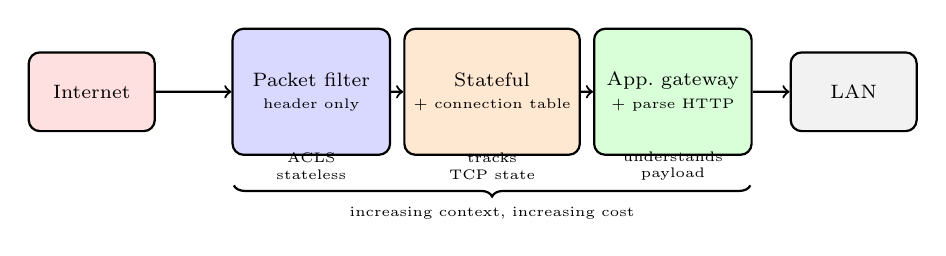
\begin{tikzpicture}[scale=0.82, every node/.style={font=\scriptsize}]
  % Left: Internet
  \node[draw,thick,fill=red!12,rounded corners,minimum width=1.6cm,minimum height=1.0cm] (inet) at (0,1.5) {Internet};
  % Three firewall stages
  \node[draw,thick,fill=blue!15,rounded corners,minimum width=2.0cm,minimum height=1.6cm,align=center] (pf) at (3.4,1.5) {Packet filter\\ \tiny header only};
  \node[draw,thick,fill=orange!18,rounded corners,minimum width=2.0cm,minimum height=1.6cm,align=center] (st) at (6.2,1.5) {Stateful\\ \tiny + connection table};
  \node[draw,thick,fill=green!15,rounded corners,minimum width=2.0cm,minimum height=1.6cm,align=center] (app) at (9.0,1.5) {App.\ gateway\\ \tiny + parse HTTP};
  \node[draw,thick,fill=gray!10,rounded corners,minimum width=1.6cm,minimum height=1.0cm] (lan) at (11.8,1.5) {LAN};
  \draw[->,thick] (inet) -- (pf); \draw[->,thick] (pf) -- (st); \draw[->,thick] (st) -- (app); \draw[->,thick] (app) -- (lan);
  \node[font=\tiny,align=center] at (3.4,0.35) {ACLS\\stateless};
  \node[font=\tiny,align=center] at (6.2,0.35) {tracks\\TCP state};
  \node[font=\tiny,align=center] at (9.0,0.35) {understands\\payload};
  \draw[decorate,decoration={brace,mirror,amplitude=4pt},thick] (2.2,0.05) -- (10.2,0.05) node[midway,below=4pt,font=\tiny] {increasing context, increasing cost};
\end{tikzpicture}}%
\caption{Firewall generations as a pipeline: each stage sees more context. Packet filters are fast but blind to state; stateful firewalls add a connection table; application gateways proxy and parse the payload.}
\label{fig:firewall-tiers}
\end{figure}

\begin{description}[leftmargin=1.2em, itemsep=0.35em]
    \item[Packet filter (stateless)] Rules match header fields only. Example ACL: \texttt{deny tcp any any eq 23} (block Telnet). Fast, cheap, but cannot tell whether a packet belongs to an established flow; must allow broad reverse rules. Implements at line rate in routers.
    \item[Stateful firewall] Maintains a \emph{state table} of active connections (SYN seen, ESTABLISHED, RELATED). Return traffic is allowed only if it matches an existing entry. E.g., allow outbound SYN, then allow inbound SYN-ACK only if a matching SYN is in the table --- blocks unsolicited inbound TCP and spoofed ACKs.
    \item[Application-layer gateway / NGFW] Terminates the connection, parses the application protocol (HTTP, DNS, SMTP), and enforces content policy: \texttt{deny http POST to /admin from !corp}, strip ActiveX, enforce TLS inspection with consent. Highest visibility, highest latency and certificate-management cost. Often called next-generation firewall (NGFW) when combined with IDS.
\end{description}

\begin{example}[Rule order matters]
Default-deny with three rules in order: (1) \texttt{allow tcp 10.0.0.0/8 any eq 443}, (2) \texttt{allow tcp any 10.0.0.5 eq 80}, (3) \texttt{deny ip any any}. A packet to \texttt{10.0.0.5:80} matches (2); if (2) were below (3) it would be dropped. First-match semantics and shadowing are a leading cause of misconfiguration. Tools like \texttt{iptables -L -n --line-numbers} help audit order.
\end{example}
Placement: packet filter at the edge router for coarse drops, stateful firewall at the perimeter, app gateway in front of web farms. Egress filtering (controlling outbound) catches compromised hosts calling home --- often more valuable than ingress rules.

\begin{remark}[DMZ]
A \emph{demilitarised zone} hosts public-facing servers between two firewalls: outer allows Internet $\to$ DMZ, inner allows DMZ $\to$ LAN only for explicitly needed flows (e.g., app $\to$ DB on 5432). Compromise of the DMZ does not directly expose the LAN.
\end{remark}

% ============================================================
\section{IDS and IPS: Signature vs.\ Anomaly}
\label{sec:ids-ips}

\begin{definition}[IDS vs.\ IPS]
An \emph{Intrusion Detection System} (IDS) is passive: it copies traffic (SPAN port or TAP), raises alerts, does not block. An \emph{Intrusion Prevention System} (IPS) is inline: it can drop, reset, or quarantine. Every IPS is an IDS that also enforces; placement determines risk of false positives becoming outages.
\end{definition}

Two detection philosophies compete.

\begin{figure}[h]\centering
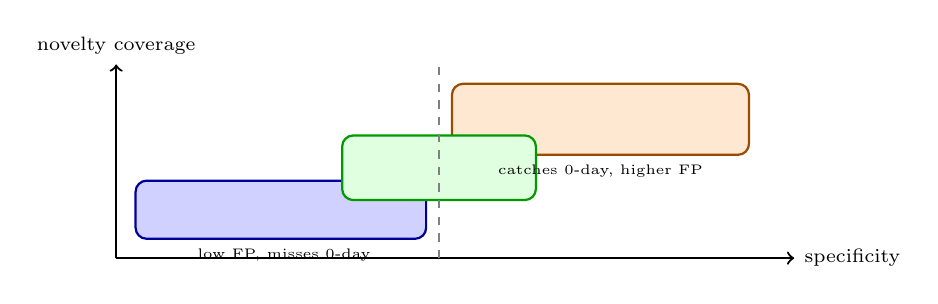
\begin{tikzpicture}[scale=0.82, every node/.style={font=\scriptsize}]
  \draw[->,thick] (0,0) -- (10.5,0) node[right] {specificity};
  \draw[->,thick] (0,0) -- (0,3.0) node[above] {novelty coverage};
  \fill[blue!18,draw=blue!60!black,thick,rounded corners] (0.3,0.3) rectangle (4.8,1.2) node[midway,align=center] {Signature\\{\tiny exact patterns, Snort rules}};
  \fill[orange!18,draw=orange!60!black,thick,rounded corners] (5.2,1.6) rectangle (9.8,2.7) node[midway,align=center] {Anomaly\\{\tiny ML / stats, deviation}};
  \fill[green!12,draw=green!60!black,thick,rounded corners] (3.5,0.9) rectangle (6.5,1.9) node[midway,align=center,font=\tiny] {hybrid};
  \node[font=\tiny,align=left] at (2.6,0.05) {low FP, misses 0-day};
  \node[font=\tiny,align=left] at (7.5,1.35) {catches 0-day, higher FP};
  \draw[dashed,gray] (5.0,0) -- (5.0,3.0);
\end{tikzpicture}
\caption{Detection trade-off. Signatures are precise but blind to novel attacks; anomaly detectors cover the unknown at the cost of more false positives. Production systems hybridise.}
\label{fig:ids-tradeoff}
\end{figure}

\begin{description}[leftmargin=1.2em, itemsep=0.35em]
    \item[Signature-based] Matches known patterns: byte sequences, regex on headers/payload, or Snort-style rules (\texttt{alert tcp any any -> any 80 (msg:"SQLi"; content:"' OR 1=1";) }). Low false positives, zero-day blind, needs frequent updates. Analogous to anti-virus signatures.
    \item[Anomaly-based] Learns a model of normal (traffic volume, n-grams, entropy, host behaviour) and flags deviation beyond a threshold. Catches novel attacks; suffers false positives and adversarial evasion (mimicry: attacker shapes traffic to look normal). Needs clean training data.
\end{description}

\begin{lstlisting}[language=Python]
# Toy signature match (IDS-style inspection)
import re
RULES = [re.compile(pat) for pat in [r"' OR 1=1", r"<script", r"\.\./"]]
def inspect(payload: str):
    for r in RULES:
        if r.search(payload):
            alert(f"signature hit: {r.pattern!r} in {payload[:80]}")
            return "ALERT"
    return "OK"
# Anomaly sketch: flag if byte-entropy deviates >3 sigma from baseline
\end{lstlisting}
Metrics: true/false positives/negatives, ROC curve. Tuning moves the threshold along the curve --- blocking (IPS) demands low false positives, so signatures dominate inline; anomaly is often alert-only for SOC analysts. Encrypted traffic blinds payload inspection, pushing detection to metadata (flow sizes, timing) and endpoints.

Placement matters: network IDS watches the wire, host IDS watches syscalls and logs. Modern EDR/XDR fuses both. An IPS that false-positives on legitimate traffic creates a self-inflicted denial of service.

% ============================================================
\section{TLS 1.3 Handshake: Whispering in Public}
\label{sec:tls13}
TLS provides confidentiality, integrity, and server (optionally client) authentication over an untrusted channel. Version 1.3 (RFC~8446) removed legacy features that caused a decade of attacks.

\begin{figure}[h]\centering
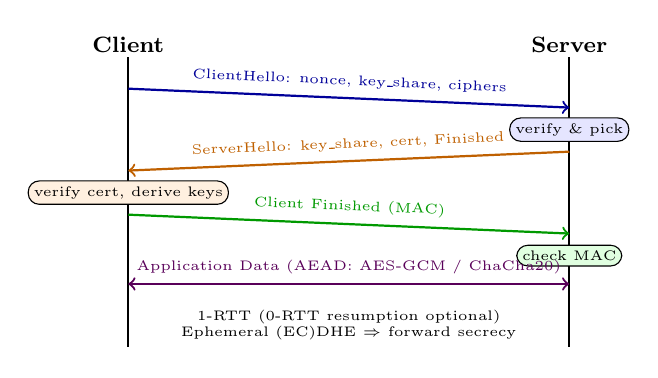
\begin{tikzpicture}[scale=0.80, every node/.style={font=\scriptsize}]
  \node[font=\footnotesize\bfseries] at (1.8,5.0) {Client}; \node[font=\footnotesize\bfseries] at (8.8,5.0) {Server};
  \draw[thick] (1.8,4.8) -- (1.8,0.2); \draw[thick] (8.8,4.8) -- (8.8,0.2);
  % 1: ClientHello
  \draw[->,thick,blue!60!black] (1.8,4.3) -- (8.8,4.0) node[midway,above,sloped,font=\tiny] {ClientHello: nonce, key\_share, ciphers};
  \node[draw,fill=blue!10,rounded corners,inner sep=2pt,font=\tiny] at (8.8,3.65) {verify \& pick};
  % 2: ServerHello
  \draw[->,thick,orange!75!black] (8.8,3.3) -- (1.8,3.0) node[midway,above,sloped,font=\tiny] {ServerHello: key\_share, cert, Finished};
  \node[draw,fill=orange!12,rounded corners,inner sep=2pt,font=\tiny] at (1.8,2.65) {verify cert, derive keys};
  % 3: Client Finished
  \draw[->,thick,green!60!black] (1.8,2.3) -- (8.8,2.0) node[midway,above,sloped,font=\tiny] {Client Finished (MAC)};
  \node[draw,fill=green!12,rounded corners,inner sep=2pt,font=\tiny] at (8.8,1.65) {check MAC};
  % Application data
  \draw[<->,thick,violet!70!black] (1.8,1.2) -- (8.8,1.2) node[midway,above,font=\tiny] {Application Data (AEAD: AES-GCM / ChaCha20)};
  \node[font=\tiny,align=center] at (5.3,0.55) {1-RTT (0-RTT resumption optional)\\Ephemeral (EC)DHE $\Rightarrow$ forward secrecy};
\end{tikzpicture}
\caption{TLS~1.3 handshake (simplified): one round trip negotiates an ephemeral Diffie--Hellman share and authenticates the server. The Finished MACs bind the transcript; everything after is AEAD-encrypted.}
\label{fig:tls13-handshake}
\end{figure}

Key ideas (intuition $\to$ formal): ephemeral \emph{(EC)DHE} means a fresh Diffie--Hellman exponent is generated per connection; the session key is $g^{xy}$ for client secret $x$ and server secret $y$. Compromise of long-term signing keys later does not reveal $x$ or $y$, so past sessions stay secret --- \emph{forward secrecy}. Contrast with RSA key transport (pre-1.3) where the session key was encrypted under the server's long-term public key: later key compromise decrypts all past sessions.

The handshake is one round trip (1-RTT); 0-RTT resumption replays a previously established PSK for speed at replay risk, so servers must enforce anti-replay (single-use tickets, freshness checks).

\begin{definition}[TLS~1.3 properties]
\emph{Authenticated key exchange} with forward secrecy; \emph{record layer} uses AEAD (AES-GCM or ChaCha20-Poly1305) for confidentiality + integrity; cipher agility is removed (only 5 suites). Handshake is encrypted after ServerHello, hiding certificates from passive observers.
\end{definition}

Certificates bind server identity to a public key via a CA chain. Client validates the chain, hostname (SAN), and expiry before deriving keys. Downgrade protection (special random values) and the \texttt{Finished} transcript MAC prevent version/cipher rollback attacks.

\begin{example}[What 1-RTT means]
Client sends key\_share $g^x$ speculatively without knowing the server's group. If the server prefers a different group, it sends \texttt{HelloRetryRequest} --- costing an extra RTT. Implementations therefore send shares for the two most likely groups (x25519, P-256).
\end{example}

% ============================================================
\section{VPNs: Private Tunnels over Public Roads}
\label{sec:vpns}
A \emph{Virtual Private Network} creates a logically private link over a public network by tunnelling and encrypting. The tunnel is a virtual point-to-point link; routing decides what enters it.

\begin{description}[leftmargin=1.2em, itemsep=0.35em]
    \item[IPSec] Network-layer suite: \emph{AH} (integrity only, now rare) and \emph{ESP} (confidentiality + integrity). Two modes: \emph{transport} (encrypts payload, keeps original IP header --- host-to-host) and \emph{tunnel} (encapsulates the entire IP packet in a new IP header --- gateway-to-gateway). Key management via \emph{IKEv2}. Used for site-to-site links and always-on corporate backhaul. Kernel-level, one SA per flow.
    \item[SSL/TLS VPN] Application-layer tunnel over TLS (often via a browser or thin client). Easier to deploy through NAT/firewalls (runs over TCP~443), supports fine-grained per-application access. Two flavours: \emph{portal} (reverse-proxy to web apps) and \emph{tunnel} (TUN/TAP adapter carrying IP). Preferred for remote-access and BYOD; user-space, firewall-friendly.
\end{description}

Think of IPSec tunnel as putting the entire letter (with its envelope) inside a new outer envelope addressed gateway-to-gateway; transport mode only seals the letter contents. TLS VPN is like accessing the office through a single HTTPS door that proxies you inside.

\begin{example}[Tunnel vs.\ transport on the wire]
Two gateways linking \texttt{10.1.0.0/16} and \texttt{10.2.0.0/16} use IPSec \emph{tunnel} mode: packet \texttt{[IP\textsubscript{inner}: 10.1.0.5$\to$10.2.0.9 | TCP]} becomes \texttt{[IP\textsubscript{outer}: GW\textsubscript{A}$\to$GW\textsubscript{B} | ESP | IP\textsubscript{inner} | TCP]} on the wire. Two laptops talking directly could use \emph{transport} mode with no outer header.
\end{example}

Comparison: IPSec excels at site-to-site (always on, transparent to apps); TLS VPN excels at road warriors (NAT traversal, per-app policy). Neither replaces endpoint security --- a compromised laptop inside the tunnel is still inside the perimeter. Split tunnelling (only corporate traffic through VPN) trades security for bandwidth and must be policy-controlled.

\begin{table}[h]\centering\small
\begin{tabular}{l l l}
\toprule & \textbf{IPSec} & \textbf{TLS VPN} \\\midrule
Layer & Network (L3), kernel & Transport/App (L4/L7), user-space \\
Through NAT & Hard (ESP, needs NAT-T) & Easy (TCP~443) \\
Client & Heavy (IKEv2, SA per flow) & Light (browser / thin agent) \\
Granularity & Per-host / per-subnet & Per-application / per-URL \\
Best for & Site-to-site, always-on & Remote access, BYOD, extranet \\\bottomrule
\end{tabular}
\caption{IPSec vs.\ TLS VPN at a glance. Choice is driven by who connects and what middleboxes lie in between.}
\end{table}

\begin{remark}[Why this all composes]
Firewalls decide \emph{whether} a packet may pass, IDS/IPS decides \emph{whether it looks malicious}, TLS decides \emph{whether anyone in the middle can read it}, and VPN decides \emph{whose network it appears to be on}. A packet from a road warrior therefore traverses: hotel NAT $\to$ TLS VPN (encrypted) $\to$ perimeter firewall (state checked) $\to$ IDS (signature scan on decrypted copy) $\to$ internal server over TLS. No single box sees everything; defence in depth does.
\end{remark}

\begin{definition}[Security association (SA)]
An \emph{SA} is the simplex state for one direction of an IPSec tunnel: encryption/integrity algorithms, keys, sequence counter, and lifetime. IKEv2 negotiates two SAs (inbound/outbound) per flow; rekeying before expiry preserves forward secrecy of the data channel.
\end{definition}

\section{Exercises}
\label{sec:ch06-exercises}
\begin{enumerate}[label=E6.\arabic*, leftmargin=*, itemsep=0.6em]
    \item \textbf{Firewall rules.} Write a default-deny ACL for a web server \texttt{203.0.113.10} that (a) allows inbound TCP~443 and 80 from anywhere, (b) allows outbound DNS (UDP~53) to \texttt{8.8.8.8}, (c) blocks Telnet (TCP~23) explicitly, (d) drops all else. Explain why the DNS rule must be stateful or paired with a reverse rule.
    \item \textbf{Stateful vs.\ stateless.} A stateless filter allows \texttt{tcp any any established}. Show how an attacker can abuse this to reach an ``established-only'' internal service by setting the ACK bit. How does a true state table prevent it? Give the exact table entry needed after a legitimate SYN.
    \item \textbf{IDS trade-offs.} A signature set has 1\% false-positive rate on 1M daily events with 10 true attacks. Compute expected alerts and precision. An anomaly detector catches 9/10 attacks at 5\% FPR. Compute its alerts and explain which is suitable for IPS blocking vs.\ IDS monitoring, using ROC intuition.
    \item \textbf{TLS~1.3 reasoning.} (a) Why does ephemeral (EC)DHE give forward secrecy while RSA key transport does not? (b) What does the \texttt{Finished} MAC cover and which attack does it prevent? (c) Why is 0-RTT replayable and what server-side mitigation is required?
    \item \textbf{VPN design.} A company needs (i) permanent link between two data centres and (ii) remote access for 500 BYOD laptops through hotel NATs. For each, choose IPSec vs.\ TLS VPN, mode (tunnel/transport/portal), and justify with firewall traversal, client provisioning, and granularity.
\end{enumerate}

\section*{Chapter Notes}
Firewalls follow Cheswick--Bellovin (1994) and the ``default deny'' doctrine; NGFW adds DPI. IDS/IPS taxonomy is Denning (1987) and Axelsson (2000); Snort/Suricata exemplify signatures, while Sommer--Paxson (2010) critiques anomaly hype. TLS~1.3 is RFC~8446 (Rescorla, 2018); prior attacks (BEAST, POODLE, Heartbleed) motivated its simplification. IPSec is RFC~4301/7296 (Kent, Kaufman); SSL VPN trade-offs are surveyed in Frankel et al.~(NIST SP~800-77).

% End of Chapter 6